


\begin{frame}{Enrichir et valider un réseau inféré}


\small Les arêtes inférées peuvent être comparées à des \textbf{liens de régulation déjà documentés}, comme :


\begin{itemize} \small 
    \item Les interactions présentes dans la \textbf{litérature}
    \item Des \textbf{données de fixation} des TFs  \textit{in vivo} ou \textit{in vitro} CHIPSeq, DAPSeq
    \item L'\textbf{accessibilité de la chromatine} et footprinting : ATACSeq
    \item La \textbf{régulation \textit{in planta}} (induction de TF dans des protoplastes \cite{Bargmann2013}, expression de gènes cibles dans des lignées de mutants, etc) 
\end{itemize}
\vspace{-0.3cm}
\onslide<2->
\begin{block}{\small Quelques efforts de regroupement en bases de données:}
\begin{itemize}\small
    \item ConnecTF \cite{Brooks2020} (Arabidopsis, maïs)
    \item AtRegNet \cite{Palaniswamy2006} (Arabidopsis)
\end{itemize}
\end{block}
\end{frame}



\begin{frame}{Enrichir et valider un réseau inféré}

\begin{columns}
\begin{column}{.5\textwidth}
\vspace{-0.1cm}
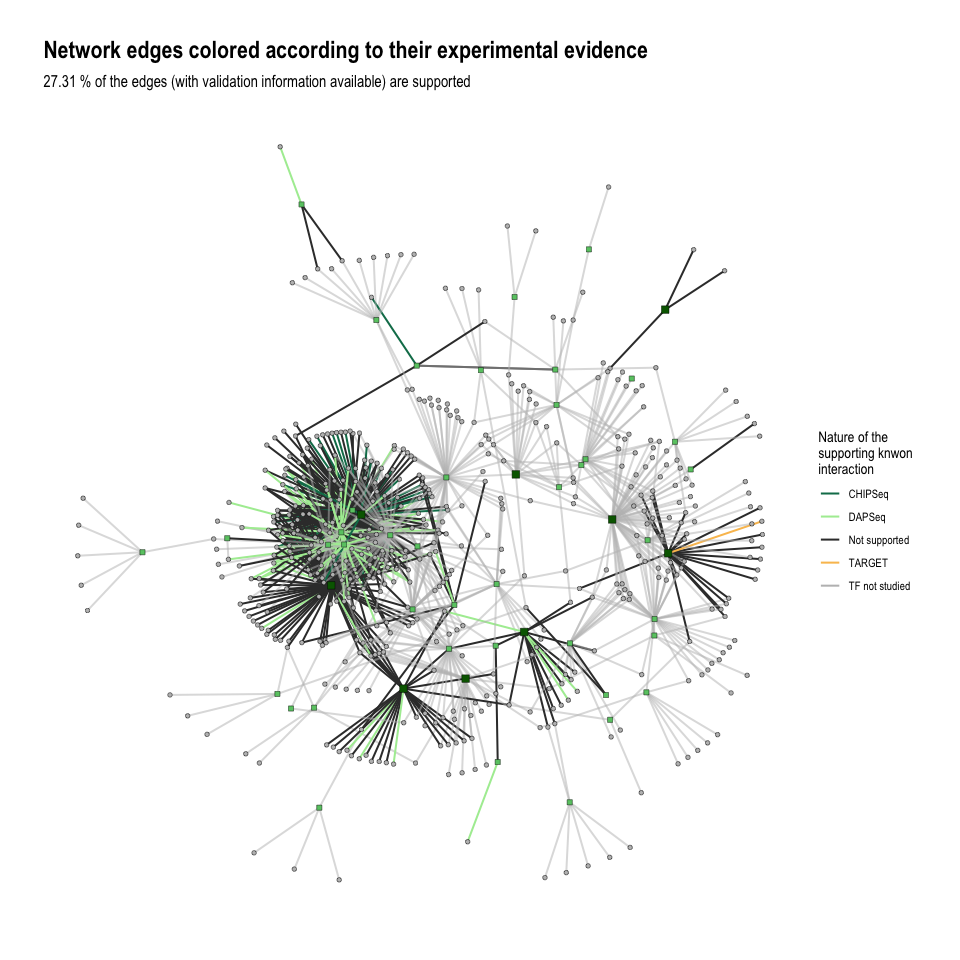
\includegraphics[scale = 0.21]{Figures/analyse/validation.png}
\end{column}
\begin{column}{.3\textwidth}
\vspace{-0.2cm}
\begin{block}{}
\scriptsize Ici, les arêtes d'un réseau prédit sont colorées suivant \textbf{leur confirmation par une expérience présente dans connecTF (DAPSeq, CHIPSeq, TARGET)}
\end{block}
\scriptsize Réseau inféré via GENIE3, validé via \href{https://oceanecsn.github.io/AraNetBench/}{AraNetBench}. \\ Arabidopsis sous stress osmotique, salin, et en température
\end{column}
\end{columns}
\end{frame}



\begin{frame}{Calculer des métriques de validation sur un réseau inféré}

\begin{columns}
\begin{column}{.48\textwidth}
\begin{itemize}\small
    \item \textbf{Vrais positifs - précision} : nombre d'arêtes prédites supportées par une information expérimentale (absolu, ou rapporté au nombre d'arêtes total qu'il est possible de valider)
    
    \item \textbf{Faux positifs, vrais négatifs, faux négatifs, rappel}
\end{itemize}
\onslide<3->
\begin{alertblock}{\small \danger Interprétation de ces métriques}\scriptsize
Ces données de validation sont \textbf{imparfaites}, elles contiennent des faux positifs, et faux négatifs : prudence
\end{alertblock}
\end{column}
\begin{column}{.48\textwidth}
\onslide<2->
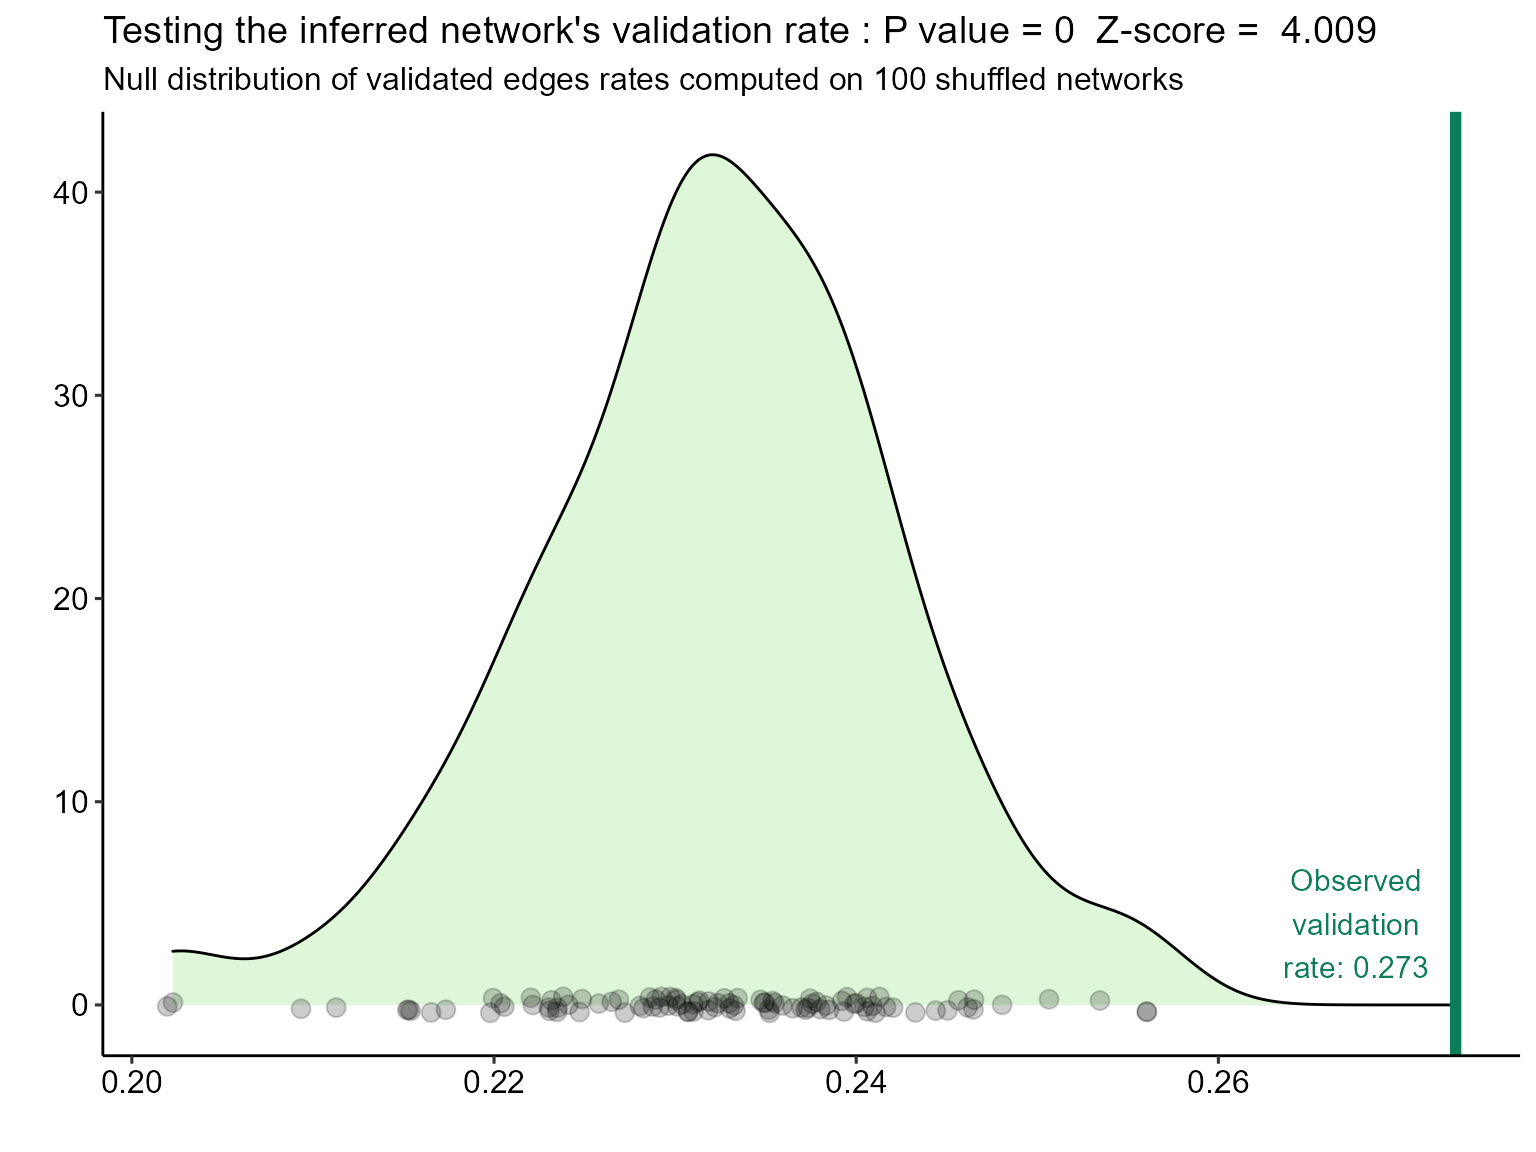
\includegraphics[scale = 0.3]{Figures/Regression/validationtest.png}
\end{column}
\end{columns}
\end{frame}
